\documentclass{report}

\usepackage{graphicx}
\usepackage{algorithm}
\usepackage{array}
\usepackage{dsfont}
\usepackage{algpseudocode}
\usepackage{listings}
\usepackage{amsmath}
\usepackage{tikz}
\usepackage{pdfpages}
\usepackage{float}

\usetikzlibrary{automata, positioning, arrows}
\DeclareMathOperator{\rank}{rank}
\makeatletter
\newenvironment{sqcases}{%
  \matrix@check\sqcases\env@sqcases
}{%
  \endarray\right.%
}
\def\env@sqcases{%
  \let\@ifnextchar\new@ifnextchar
  \left\lbrack
  \def\arraystretch{1.2}%
  \array{@{}l@{\quad}l@{}}%
}
\makeatother

\usetikzlibrary{calc}


\input{/mnt/fa80f336-3342-4d78-8bfd-a43e434a2cda/Latex/preamble.tex}
\input{/mnt/fa80f336-3342-4d78-8bfd-a43e434a2cda/Latex/macros.tex}
\input{/mnt/fa80f336-3342-4d78-8bfd-a43e434a2cda/Latex/letterfonts.tex}

\title{\Huge{FU08 \-- Automata and Languages}\\Exercise 8}
\author{\huge{NGUYEN Tuan Dung}\\\huge{s1312004}}
\date{January 14, 2025}

\begin{document}

\maketitle

% Cau 1
\qs{Construct a DFA that accepts the language generated by the grammar}{
$ \mathrm{S} \longrightarrow \mathrm{abA,}\\
\mathrm{A} \longrightarrow \mathrm{baB,}\\
\mathrm{B} \longrightarrow \mathrm{aA|bb}
$}

\sol{\newline
\\
\begin{minipage}[t]{0.48\textwidth}
We sketch the DFA out, with the start state S, final state F.\\
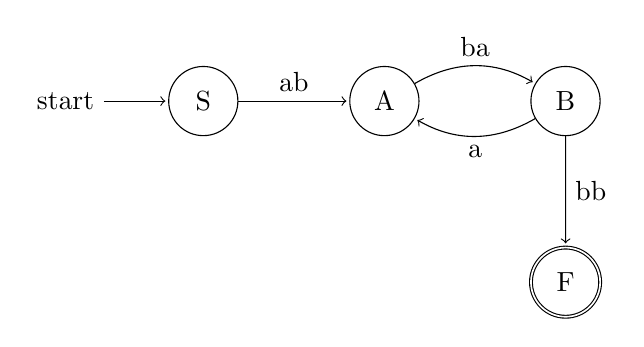
\begin{tikzpicture}[shorten >=1pt, scale=1.8, node distance=2.3cm, on grid, auto][h]
    \node[state, initial] (s) {S};
    \node[state] (a) [right=of s] {A};
    \node[state] (b) [right=of a] {B};
    \node[state, accepting] (f) [below of=b] {F};

    \path[->]   
    (s) edge node {ab} (a)
    (a) edge[bend left] node {ba} (b)
    (b) edge[bend left] node {a} (a)
        (b) edge node {bb} (f);
\end{tikzpicture}
\end{minipage}
\hfill
\begin{minipage}[t]{0.48\textwidth}
Split the transitions, we obtain the final DFA.\\
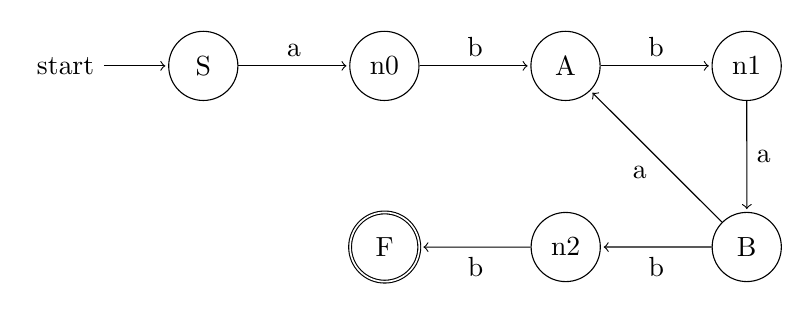
\begin{tikzpicture}[shorten >=1pt, scale=1.8, node distance=2.3cm, on grid, auto][h]
    \node[state, initial] (s) {S};
    \node[state] (n0) [right=of s] {n0};
    \node[state] (a) [right=of n0] {A};
    \node[state] (n1) [right=of a] {n1};
    \node[state] (b) [below of=n1] {B};
    \node[state] (n2) [left=of b] {n2};
    \node[state, accepting] (f) [left=of n2] {F};

    \path[->]  
    (s) edge node {a} (n0)
    (n0) edge node {b} (a)
    (a) edge node {b} (n1)
    (n1) edge node {a} (b)
    (b) edge node {a} (a)
        (b) edge node {b} (n2)
    (n2) edge node {b} (f);
\end{tikzpicture}
\end{minipage}
\newline
\\
\noindent Fast conversion from DFA to regular expression, we obtain $\mathrm{abba(aba)}^*\mathrm{bb}$.
}
\newline
\\

% Cau 2
\qs{Construct right- and left-linear grammars for the language}{
$L = \{a^nb^m : n \geq 2, m \geq 3\}$
}

\sol{\newline
\\
Fast conversion to regular expression, we obtain $\mathrm{aaa}^*\mathrm{bbbb}^* = \mathrm{aaa}^*\mathrm{b}^*\mathrm{bbb}$.\\
\begin{minipage}[t]{0.48\textwidth}
$\bullet$ Right-linear grammar: start from left to right\newline
$\mathrm{S} \longrightarrow \mathrm{aaA}\\
\mathrm{A} \longrightarrow \mathrm{aA|B}\\
\mathrm{B} \longrightarrow \mathrm{bbbC}\\
\mathrm{C} \longrightarrow \mathrm{bC|}\lambda
$
\end{minipage}
\hfill
\begin{minipage}[t]{0.48\textwidth}
$\bullet$ Left-linear grammar: start from right to left\newline
$\mathrm{S} \longrightarrow \mathrm{Abbb}\\
\mathrm{A} \longrightarrow \mathrm{Ab|B}\\
\mathrm{B} \longrightarrow \mathrm{Caa}\\
\mathrm{C} \longrightarrow \lambda
$
\end{minipage}
}
\newline
\\
% Cau 3
\qs{Answer the following question}{
Construct right- and left-linear grammars for the language generated by the following regular expression.
\newline
$\mathrm{r} = (\mathrm{aab}^*\mathrm{ab})^*$
}

\sol{\newline
\\
\begin{minipage}[t]{0.48\textwidth}
$\bullet$ Right-linear grammar: start from left to right\newline
$\mathrm{S} \longrightarrow \lambda\mathrm{|aaA}\\
\mathrm{A} \longrightarrow \mathrm{bA|abS}
$
\end{minipage}
\hfill
\begin{minipage}[t]{0.48\textwidth}
$\bullet$ Left-linear grammar: start from right to left\newline
$\mathrm{S} \longrightarrow \lambda\mathrm{|Aab}\\
\mathrm{A} \longrightarrow \mathrm{Ab|Saa}
$
\end{minipage}
\newline
\\
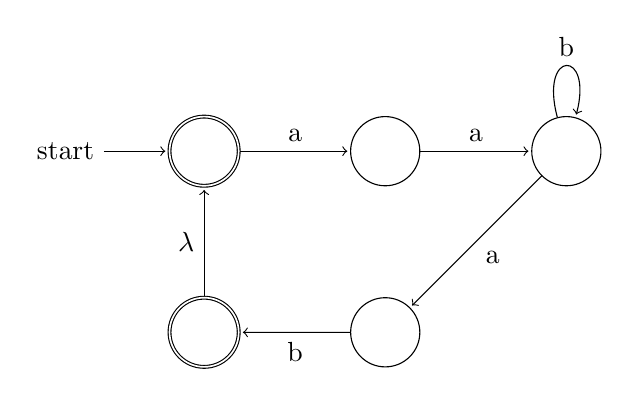
\begin{tikzpicture}[shorten >=1pt, scale=1.8, node distance=2.3cm, on grid, auto][h]
    \node[state, initial, accepting] (0) {};
    \node[state] (1) [right=of 0] {};
    \node[state] (2) [right=of 1] {};
    \node[state] (3) [below of=1] {};
    \node[state, accepting] (4) [below of=0] {};

    \path[->]  
    (0) edge node {a} (1)
    (1) edge node {a} (2)
    (2) edge[loop above] node {b} (2)
        (2) edge node {a} (3)
    (3) edge node {b} (4)
    (4) edge node {$\lambda$} (0);
\end{tikzpicture}
}

\pagebreak

% Cau 4
\qs{Construct a context-free grammar for the language}{
    \{$\mathrm{a}^i\mathrm{b}^j\mathrm{c}^k\mathrm{~:i} \neq \mathrm{j~or~j} \neq \mathrm{k}$\}\\
that is the language of strings of a's followed by b's followed by c's, such that there are either a different number of a's and b's or a different number of b's and c's, or both.
}

\sol{\newline
\\
\noindent Since i $\neq$ j or j $\neq$ k $\Leftrightarrow$ i $<$ j or i $>$ j or j $>$ k or j $<$ k.\\
\\
$\mathrm{S} \longrightarrow \mathrm{X_{i<j}C~|~X_{i>j}C~|~AY_{j<k}~|~AY_{j>k}}\\
\\
\mathrm{A} \longrightarrow \mathrm{aA~|~}\lambda\\
\mathrm{B} \longrightarrow \mathrm{bB~|~}\lambda\\
\mathrm{C} \longrightarrow \mathrm{cC~|~}\lambda\\
\\
\mathrm{X_{i>j}} \longrightarrow \mathrm{aX_{i>j}b~|~aA}\\
\\
\mathrm{X_{i<j}} \longrightarrow \mathrm{aX_{i<j}b~|~bB}\\
\\
\mathrm{Y_{j<k}} \longrightarrow \mathrm{bY_{j<k}c~|~cC}\\
\\
\mathrm{Y_{j>k}} \longrightarrow \mathrm{bY_{j<k}c~|~bB}
$
}
\end{document}
